\documentclass{beamer}\usetheme{boxes}

\usepackage{amsmath,hyperref,multimedia}

\newcommand{\Mp}{\ensuremath{{M_{+}}}}
\newcommand{\barMp}{\ensuremath{\overline{\Mp}}}
\newcommand{\Dt}{\ensuremath{\Delta t}}
\newcommand{\tM}[1]{\ensuremath{\tilde{M}(#1)}}
\newcommand{\tMt}{\tM{\tau}}
\newcommand{\tMB}{\ensuremath{{\tilde{M}_B}}}
\newcommand{\tE}[1]{\ensuremath{{\tilde{E}(#1)}}}
\newcommand{\tEt}{\tE{\tau}}

\newcommand{\bskip}{\\~\\}
\usepackage{Sweave}
\begin{document}
\input{sunbelt13-pres-concordance}
\title{Detection of Small Covert Networks Embedded in Large Networks}
\author{Carl~A.~B.~Pearson\inst{1} \and Burton H. Singer\inst{1} \\~\\ \and Edo Airoldi\inst{2} \and Ed Kao\inst{2}}
\institute{Emerging Pathogens Institute, University of Florida\inst{1} \and Statistics, Harvard University\inst{2}}
\frame{\titlepage}

\usebackgroundtemplate{
\vbox to \paperheight{\vfil\hbox to \paperwidth{\hfil
\includegraphics[width=0.7\paperheight,height=0.7\paperheight]{2012army.png}\hfil}\vfil} }
\frame{
\frametitle{Brought to you by Award \#W911NF-11-1-0036Z}
}
\usebackgroundtemplate{}

\frame{
\frametitle{Overview}
\begin{itemize}
\item Definitions,
\item A Model to Reflect Those,
\item A Particular Implementation: Salafi Jihadi Network,
\item Strategies for Detecting Groups,
\item Some Results, and
\item Flaws, Extensions, and Outlook
\end{itemize}
}

\frame{
\begin{block}{What is {\em Covert}?}
{\em a covert network} is a sub graph where edge information is unavailable, unreliable, or indistinguishable from whole graph structure - but that sub graph is informative
\end{block}
\begin{block}{\ldots or Operationally}
A relatively small, organized group of conspirators, masking their existence via communication discipline and taking advantage of a noisy background, who are preparing some event.

For this particular talk: Salafi Jihadi network as described by Sageman, et al\cite{qin2005analyzing}.

Note: not that group's more recent focus on {\em leaderless jihad}.
\end{block}
}

\usebackgroundtemplate{
\vbox to \paperheight{\vfil\hbox to \paperwidth{\hfil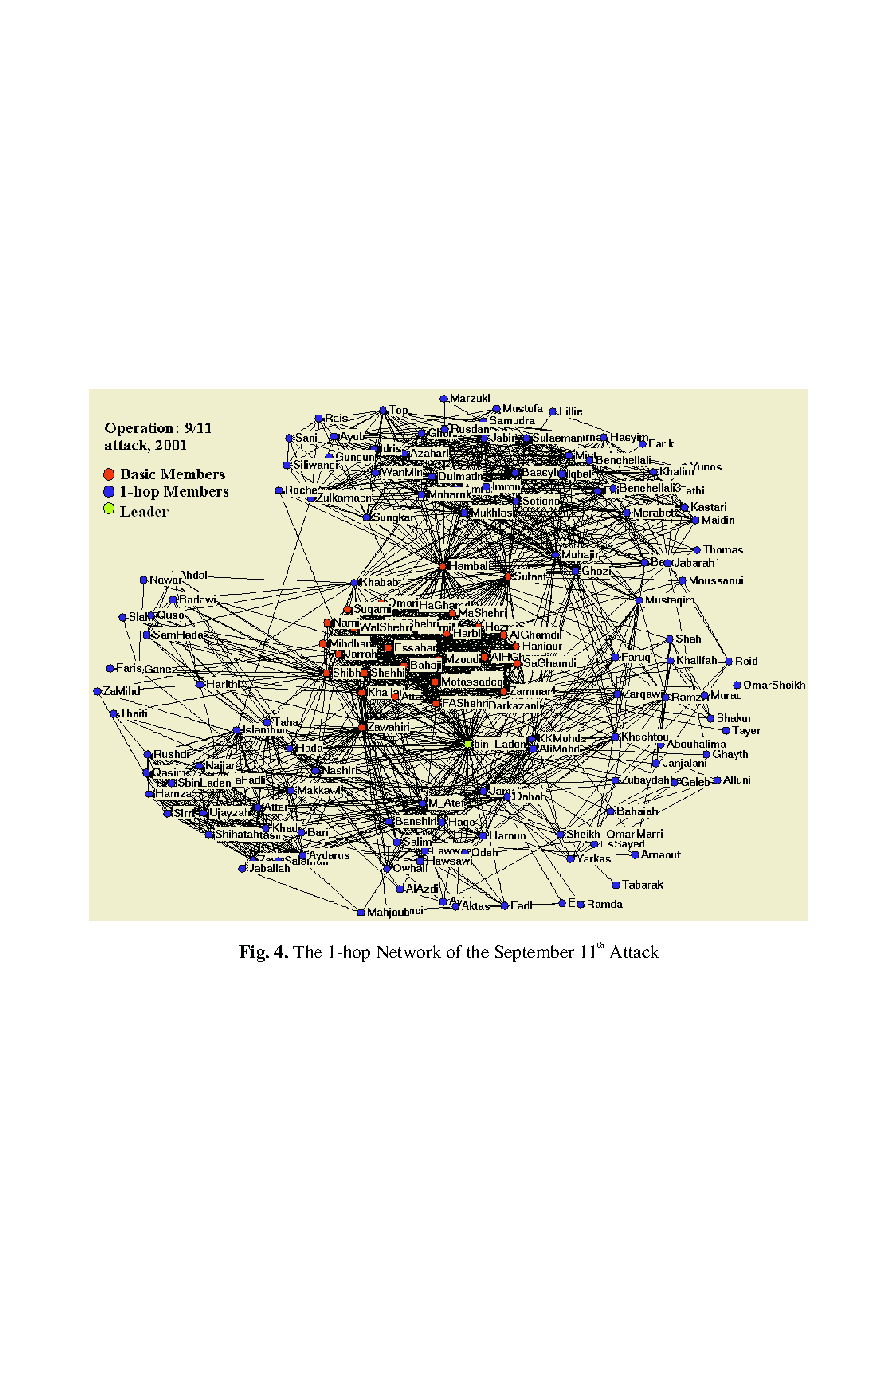
\includegraphics[width=0.9\paperheight,height=0.9\paperheight]{sageman_crop.pdf}\hfil}\vfil} }
\frame{}
\usebackgroundtemplate{}

\frame{
\begin{block}{Salient Features}
\begin{itemize}
\item highly interconnected subordinate groups, and
\item bridging middle managers,
\item communications masked with some tradecraft,
\item missing from picture: vast background population
\end{itemize}
\end{block}
}

\frame{
\frametitle{Simple Implementation addressing a Salafi Jihadi-like Network}
\begin{description}
\item[background population] many small cliques, which are recursively cliqued into single graph
\item[covert leader] embedded in background, with connections to subordinate groups
\item[subordinates] few, medium size cliques with connections between clusters
\item[communications] simple message content {\em Good} vs. {\em Bad}
\end{description}
}

\frame{
\frametitle{\ldots or Symbolically}
\begin{itemize}
\item a structured population, $P$,
\item covert leader, $H$,
\item subordinate covert groups, $\{C_i\}$,
\item stochastic behavior model for intra- and inter-group messages,
\item drawn from a set vocabulary, $V$
\end{itemize}
}

\frame{
\frametitle{Aside: Sales Pitch}
Scala-based Implementation available for review/remix:
\bskip
\href{https://github.com/pearsonca/scala-commsim}{https://github.com/pearsonca/scala-commsim}
\bskip
Actively moving from closed, non-Scala implementation to that repository.  Please request changes, point out bugs, etc.
\bskip
Also, this presentation:
\bskip
\href{https://github.com/pearsonca/sunbelt13-presentation}{https://github.com/pearsonca/sunbelt13-presentation}
}

\frame[c]{
{\center Some Networks Generated By This Procedure...}
}

\usebackgroundtemplate{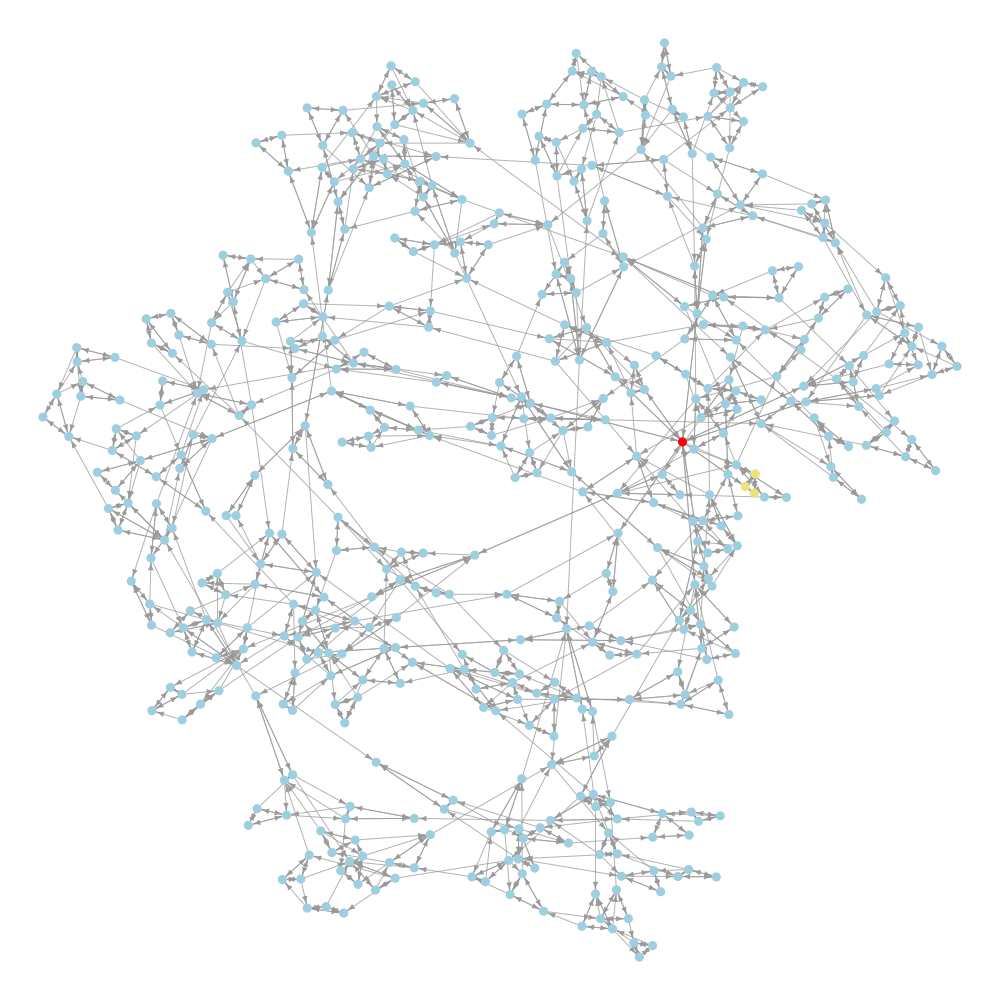
\includegraphics[width=0.9\paperheight,height=0.9\paperheight]{3_1_500.png}}
\frame{
\begin{columns}[t]
\begin{column}{0.7\textwidth}\end{column}
\begin{column}{0.3\textwidth}
3 clique, 1\%\ remix
\end{column}
\end{columns}
}
\usebackgroundtemplate{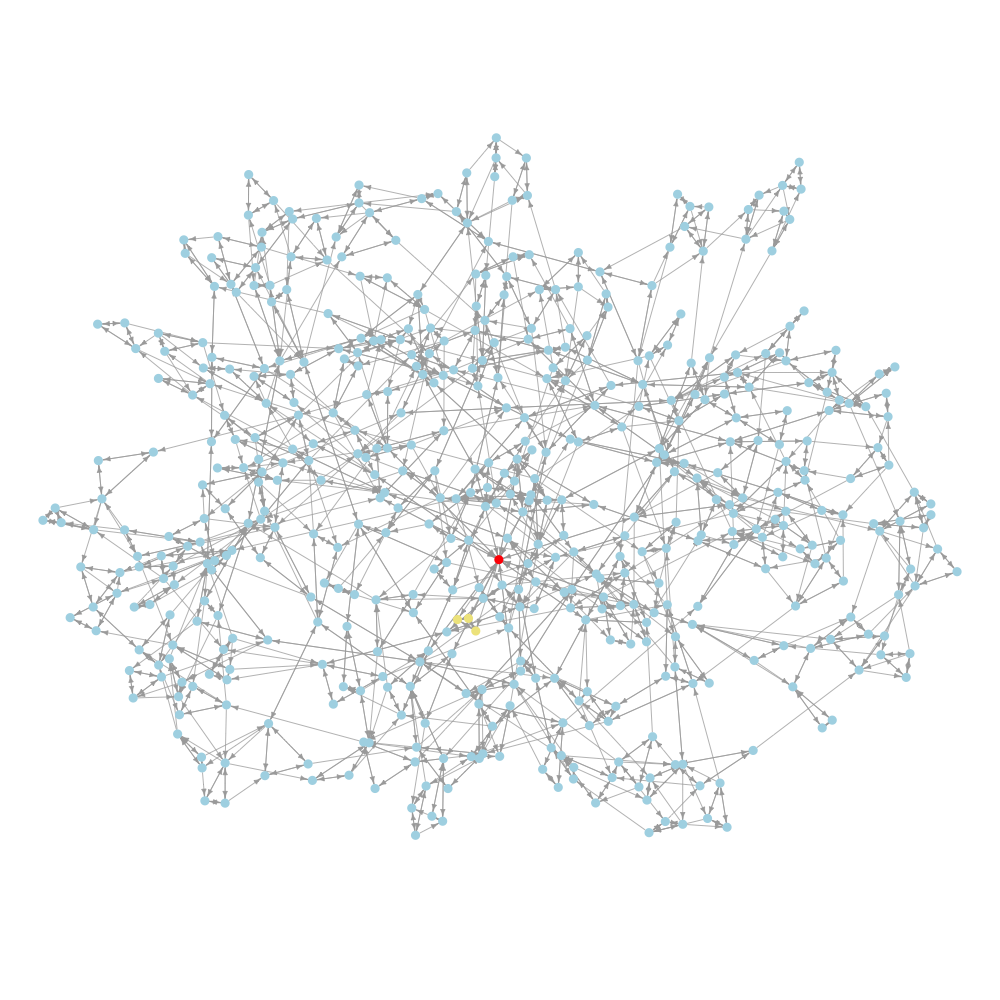
\includegraphics[width=0.9\paperheight,height=0.9\paperheight]{3_10_500.png}}
\frame{
\begin{columns}[t]
\begin{column}{0.7\textwidth}\end{column}
\begin{column}{0.3\textwidth}
3 clique, 10\%\ remix
\end{column}
\end{columns}
}
\usebackgroundtemplate{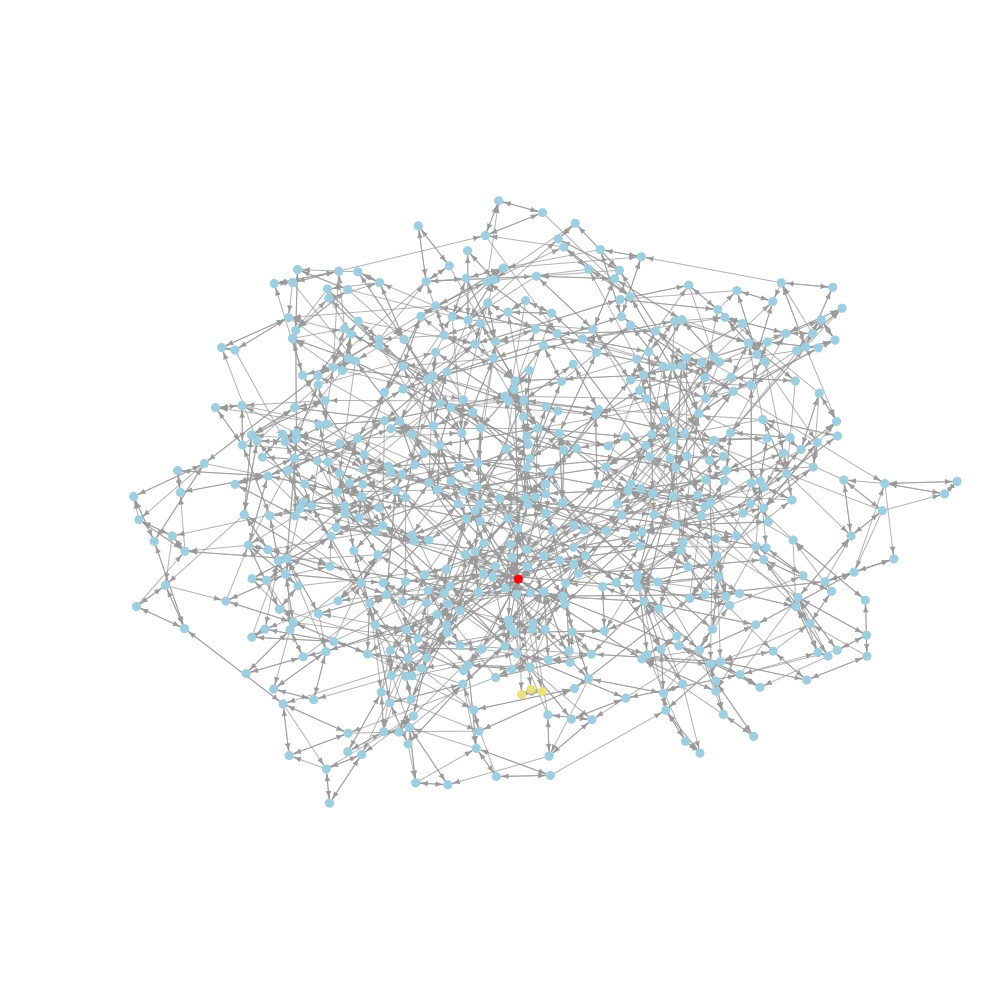
\includegraphics[width=0.9\paperheight,height=0.9\paperheight]{3_30_500.png}}
\frame{
\begin{columns}[t]
\begin{column}{0.7\textwidth}\end{column}
\begin{column}{0.3\textwidth}
3 clique, 30\%\ remix
\end{column}
\end{columns}
}
\usebackgroundtemplate{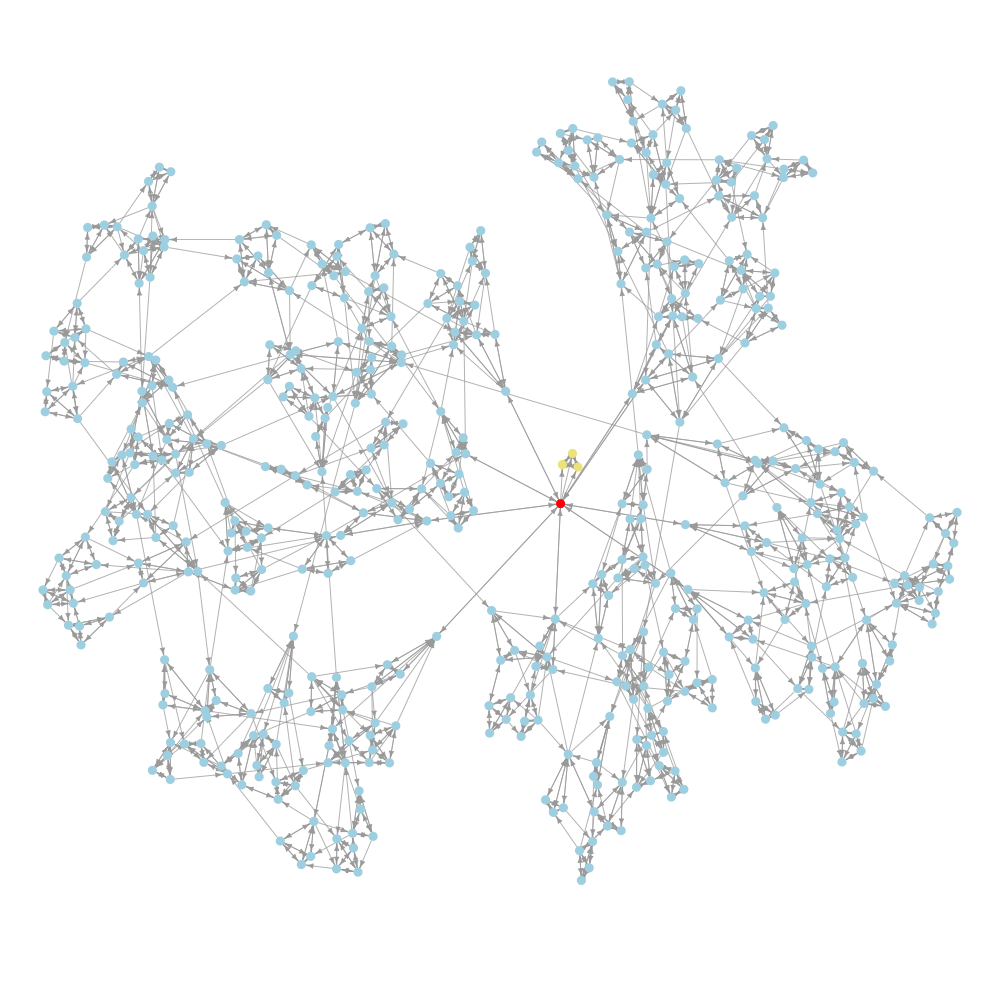
\includegraphics[width=0.9\paperheight,height=0.9\paperheight]{4_1_500.png}}
\frame{
\begin{columns}[t]
\begin{column}{0.7\textwidth}\end{column}
\begin{column}{0.3\textwidth}
4 clique, 1\%\ remix
\end{column}
\end{columns}
}
\usebackgroundtemplate{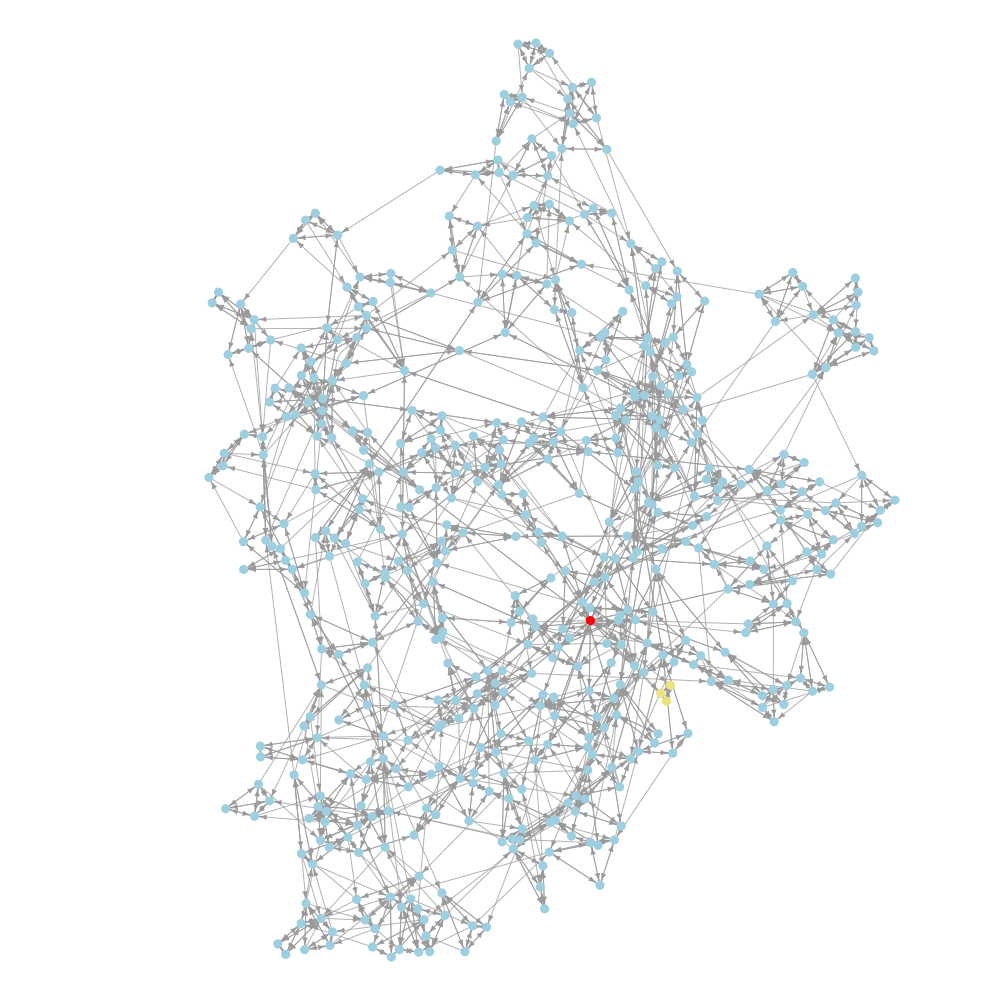
\includegraphics[width=0.9\paperheight,height=0.9\paperheight]{4_10_500.png}}
\frame{
\begin{columns}[t]
\begin{column}{0.7\textwidth}\end{column}
\begin{column}{0.3\textwidth}
4 clique, 10\%\ remix
\end{column}
\end{columns}
}

\usebackgroundtemplate{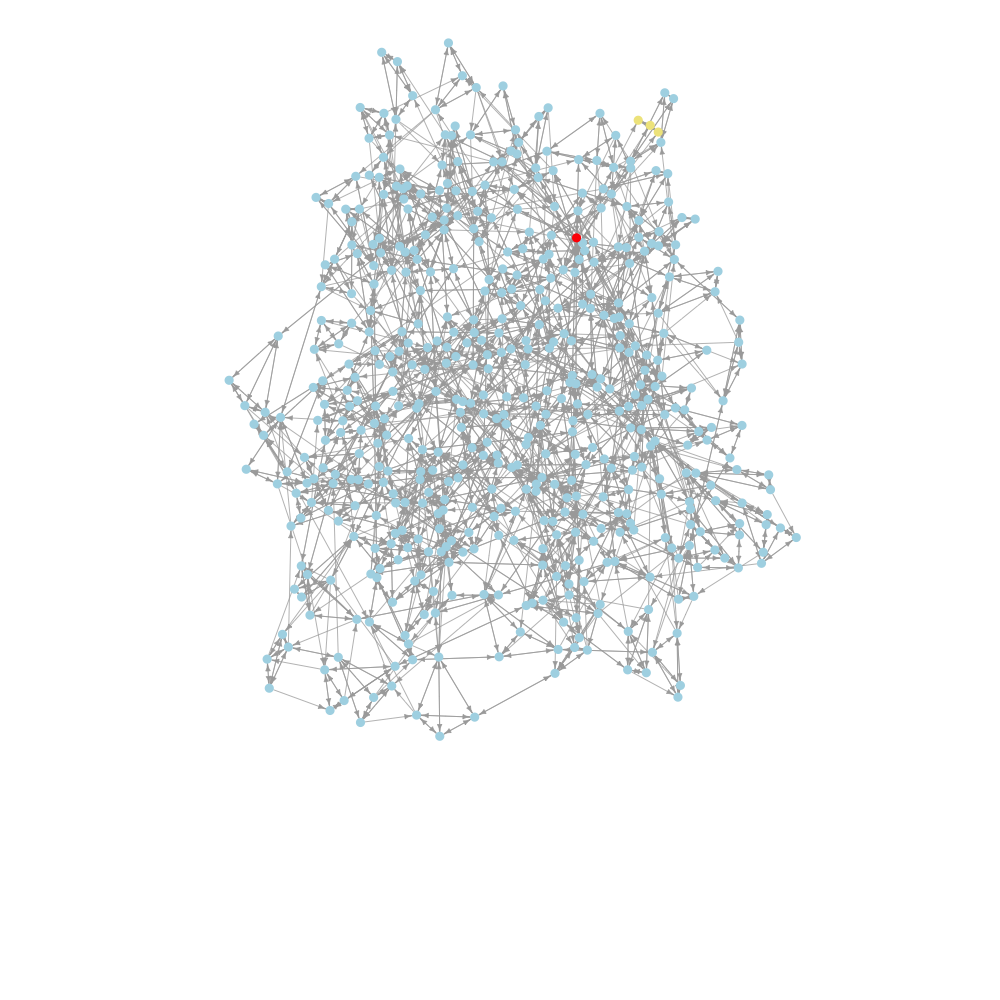
\includegraphics[width=0.9\paperheight,height=0.9\paperheight]{4_30_500.png}}
\frame{
\begin{columns}[t]
\begin{column}{0.7\textwidth}\end{column}
\begin{column}{0.3\textwidth}
4 clique, 30\%\ remix
\end{column}
\end{columns}
}
\usebackgroundtemplate{}

\frame{
\frametitle{Steady State, Structural View vs. Real Time}
\movie[externalviewer]{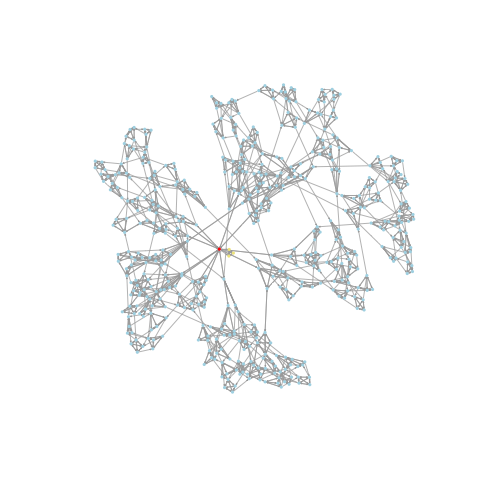
\includegraphics[width=0.9\paperheight,height=0.9\paperheight]{testoverlay.png}}{timeseries.mp4}
}

\frame{
\frametitle{Real Time Challenges to Detection}
\begin{itemize}
\item population vs. covert group communication network initially unknown,
\item potentially limited resources for monitoring those communications,
\item thus gathered information unreliable / incomplete,
\item and risk trade-offs: FPR \&\ TPR vs. action by group
\end{itemize}
% notes-notes-notes
}

\frame{
\frametitle{Detection Model: The Observer}
An algorithmic description of
\begin{itemize}
\item the data limitations (e.g., random suppression or transformation of signals), and
\item detection strategy(ies)
\end{itemize}
}

\frame{
\frametitle{Some Simple Strategies}
\begin{itemize}
\item pure content: pick up everyone that has sent and received a {\em Bad} message
\item pure structural: pick up highest degree person and all people below median
\item mixed structural and content
\end{itemize}
}

\frame{
\frametitle{Appropriate Measures?}
Assume that any given plot has some critical amount of planning-related communication.

But what else?
\begin{itemize}
\item true positive rate,
\item false positive rate,
\item resource investment
\end{itemize}

% not obvious how to transform planning-related communication rate, so use a post for the other TPR, FPR
}


\usebackgroundtemplate{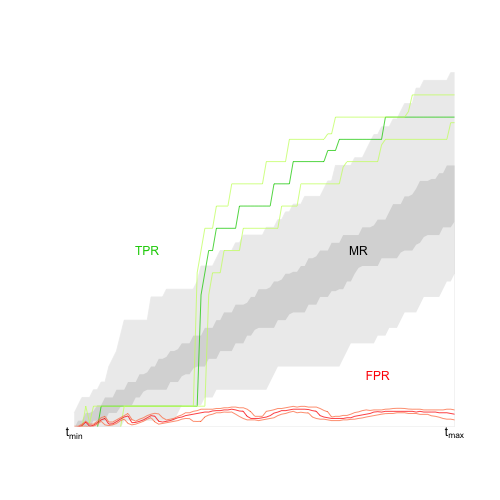
\includegraphics[width=0.9\paperheight,height=0.9\paperheight]{4_1_500_s.png}}
\frame{
\begin{columns}[t]
\begin{column}{0.7\textwidth}\end{column}
\begin{column}{0.3\textwidth}
structural only
\end{column}
\end{columns}
}
\usebackgroundtemplate{}

\usebackgroundtemplate{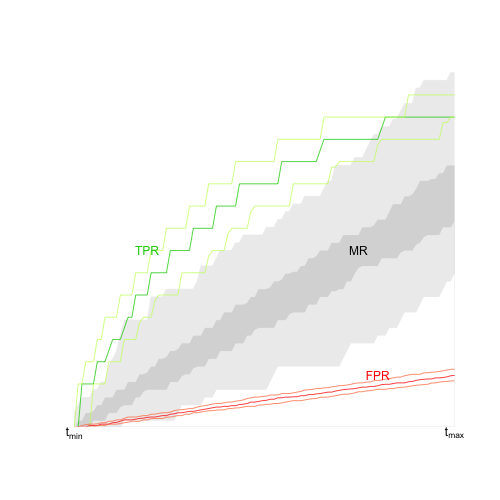
\includegraphics[width=0.9\paperheight,height=0.9\paperheight]{4_1_500_c.png}}
\frame{
\begin{columns}[t]
\begin{column}{0.7\textwidth}\end{column}
\begin{column}{0.3\textwidth}
content only
\end{column}
\end{columns}
}
\usebackgroundtemplate{}

\usebackgroundtemplate{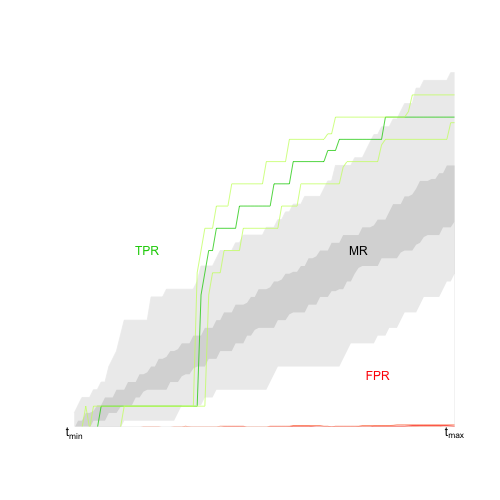
\includegraphics[width=0.9\paperheight,height=0.9\paperheight]{4_1_500_sandc.png}}
\frame{
\begin{columns}[t]
\begin{column}{0.7\textwidth}\end{column}
\begin{column}{0.3\textwidth}
structure + content
\end{column}
\end{columns}
}
\usebackgroundtemplate{}

\frame{
\frametitle{Flaws, Extensions, and Outlook}
\begin{itemize}
\item limited vocabulary -- add message diversity, require content detection as well,
\item unsophisticated Observer model and strategies -- add resource model, shifting strategies
\item background / foreground structural generations -- new generators, fitting to live traffic
\item integrate additional relationship types -- demo only uses ``Family'' and ``Plot'' contexts
\end{itemize}
}

\frame{\footnotesize
\bibliography{sageman}{}
\bibliographystyle{plain}
}

\end{document}
